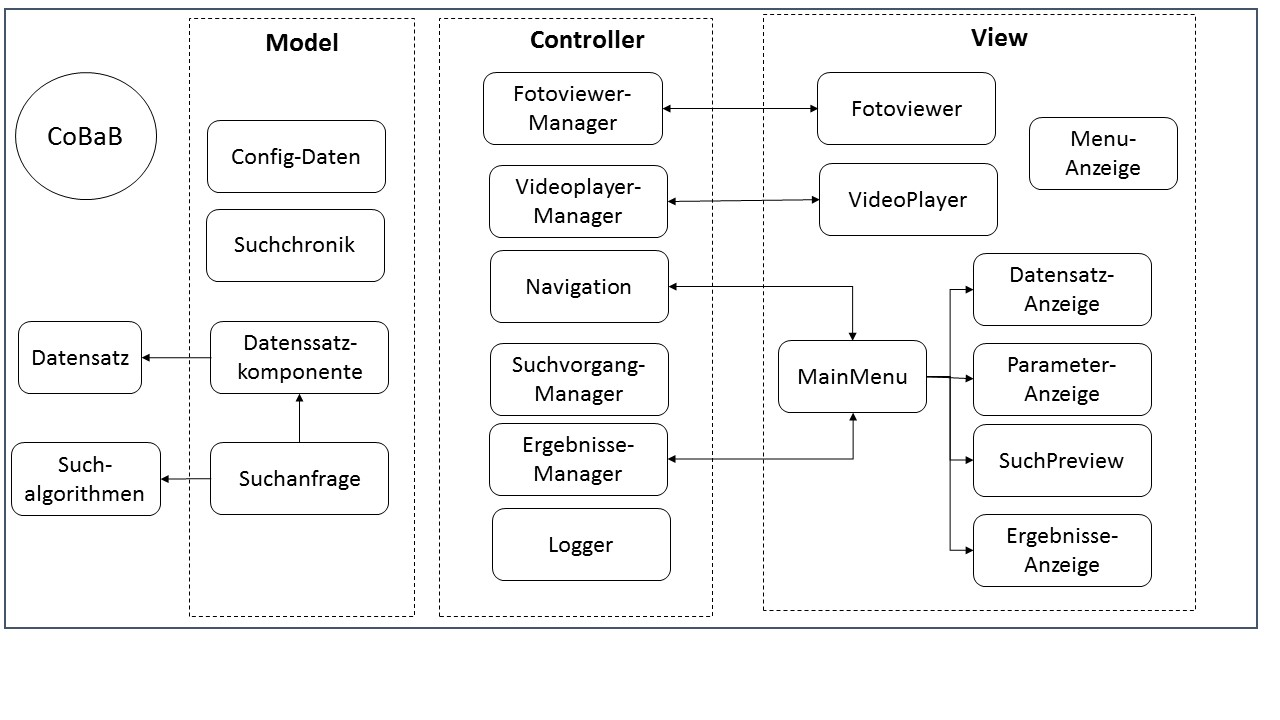
\includegraphics[width=1\linewidth]{img/SystemModell}
Die Grundstruktur des Programm folgt dem Prinzip der MVC-Architektur. Die Unterteilung der Submodule in Modell, View und Controller soll eine leichte Modifikation und Erweiterung unter anderen Platformen ermöglichen.

\begin{itemize}
\item Datensatz\newline
Die Bilder und Videos bilden eine Grundlage der Anwendung, außerdem werden auch die Annotationen gespeichert.
\item Datensatzschnittstelle\newline
Die Datensatzschnittstelle bietet sowohl der Anwendung als auch den Suchverfahren einen einheitlichen Zugriff auf die hinterlegten Daten. Diese Schnittstelle wird von der Datensatzkomponente implementiert.
\item Suchalgorithmen\newline
Verschiedene austauschbare inhaltsbasiert Suchalgorithmen. Unter eine wohldefinierte Schnitstelle kann CoBaB die Algorithmen verwenden.
\item Suchschnittstelle\newline
Die Suchschnittstelle ermöglicht eine einheitliche Verwendung der Suchalgorithmen.
\end{itemize}

\subsection{Model}
\begin{itemize}
\item Konfigurationsdaten\newline
Die Konfigurationsdaten passen die Anwendung an die Präferenzen des Benutzers an: Die gewählte Sprache und die Aktivierung bzw. Deaktivierung des Benachrichtigungstons werden gespeichert und beim erneuten Starten der Anwendung als Voreinstellung gesetzt. Außerdem wird eine Hilfe-Datei gespeichert.
\item Datensatzkomponente\newline
Die Datensatzkomponente implementiert die Datensatzschnittstelle, um auf die Bilder bzw. Videos zuzugreifen.
\item Suchanfrage\newline
Die Anwendung generiert eine Suchanfrage, die aus gewähltem Suchvorlage, gewünschtem Suchverfahren, den Suchparametern und dem Suchraum besteht. Der Suchraum ist durch den Datensatz festgelegt, in dem gesucht werden soll.
\item Suchchronik\newline
Der Benutzer kann sich die letzten Suchergebnisse anzeigen lassen und außerdem Lesezeichen für spezielle Ergebnisse speichern.
\end{itemize}

\subsection{View}
\begin{itemize}
\item Mainwindow \newline
Das Mainwindow ist beim Starten des Programms zu sehen. Anfangs ist nur eine voreingestellte Auswahl an Datensätzen zu sehen.Jedes mal beim erneuten Öffnen werden die zuletzt genutzten Datensätze angezeigt. Man kann entweder einen Datensatz aus den angezeigten wählen oder über einen Auswahl-Dialog einen neuen suchen.
\item Menü-Anzeige \newline
Das Menü beinhaltet Bequemlichkeitsfunktionen wie \textbf{Datei}, wo zusätzliche Das Beenden des Programms und die Datensatzauswahl ermöglicht ist, \textbf{Sprachauswahl}, \textbf{Hilfe}, wo es Informationen über das Programm gibt oder Anweisungen zum Benutzen der Anwendung, \textbf{Chronik} mit gespeicherten früheren Suchen, \textbf{Lesezeichen}, die der Benutzer selbst aus seinen Suchergebnissen herstellt.
\item Fotoviewer \newline
Die Fotoviewer erlaubt das Browsen durch die Fotos des gewählten Datensatzes mit bekannten Funktionen wie \enquote{voriges}, \enquote{nächstes}, Zoom und Vollbildmodus. Es gibt zusätzlich eine Option zum Wählen eines bestimmten Bereichs des Bildes. Durch einen Rechtsklick bestimmt man das Suchverfahren, das auf das Foto angewendet wird.
\item Videoplayer \newline
Der Videoplayer ist ähnlich der Foto-Anzeige aufgebaut, zuzüglich üblicher Funktionen zum Abspielen und Pausieren.
\item Datensatzanzeige \newline

\item Ergebnisseanzeige \newline


%\item Datensatzauswahl \newline
%Die Datensatzauswahl stellt ein Dialogfenster dar. Hier kann ein Datensatz aus den verfügbaren ausgewählt werden.
\end{itemize}
\item FotoViewerManager \newline
\item VideoplayerManager \newline
\item Navigation \newline
\item SuchvorgangManager \newline
\item ErgebnisseManager \newline
\item Logger \newline


\subsection{Controller}
\begin{itemize}

\end{itemize}

\pagebreak
